% this file is called up by thesis.tex
% content in this file will be fed into the main document
\ifpdf
    \graphicspath{{5/figures/PNG/}{5/figures/PDF/}{5/figures/}}
\else
    \graphicspath{{5/figures/EPS/}{5/figures/}}
\fi

\chapter{Optimization/Automatic Design of a HYDROMATRIX\circledR Turbine} % top level followed by section, subsection
Hydromatrix$\circledR$ is an axial reaction type water turbine (fig.\ref{Matrix_c}) developed by ANDRITZ HYDRO GmbH as an innovative solution for the development of low head hydropower sites \cite{matrix,matrix_2}. The concept behind Hydromatrix$\circledR$  idea is the use of a number of small non-regulated (fixed-blade) turbines in the place of a conventional large regulated one (fig.\ref{Matrix_a}) .  Regulation of a Hydromatrix$\circledR$ system can be achieved via closing/opening a number of turbines so to keep the massflow per open turbine as close as possible to there design point. If the flow exceeds the capacity, to avoid flood, a number of turbines can be raised or removed from its operating position like a gate (fig.~\ref{Matrix_a}).  


\begin{figure}[h!]
\begin{minipage}[b]{0.5\linewidth}
 \centering
 \resizebox*{7.0cm}{!}{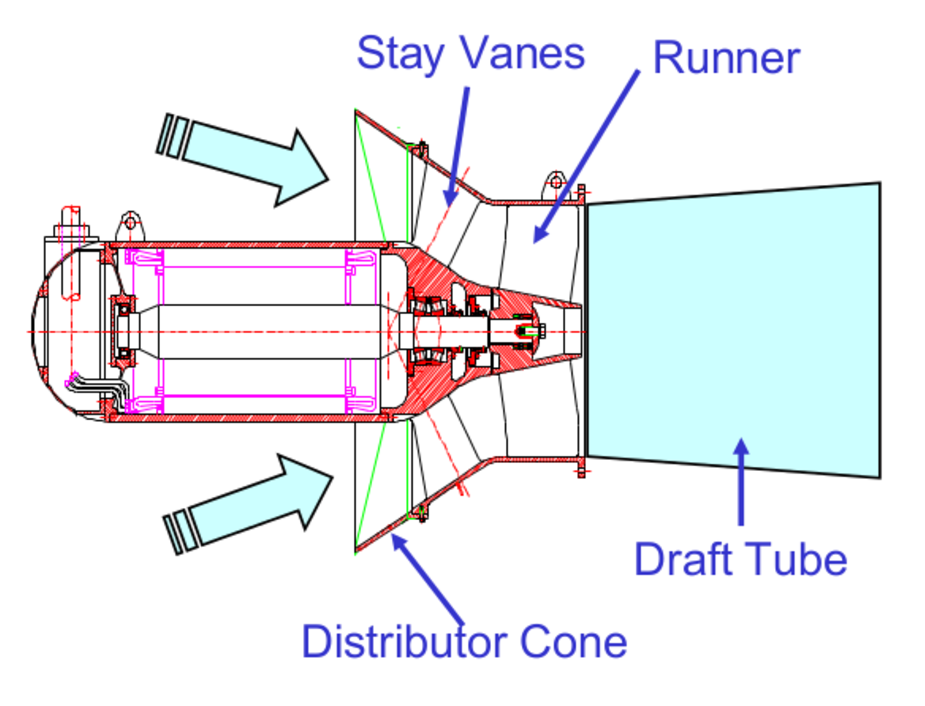
\includegraphics{Matrix1.eps}}
\end{minipage}
\begin{minipage}[b]{0.5\linewidth}
 \centering
 \resizebox*{7.0cm}{!}{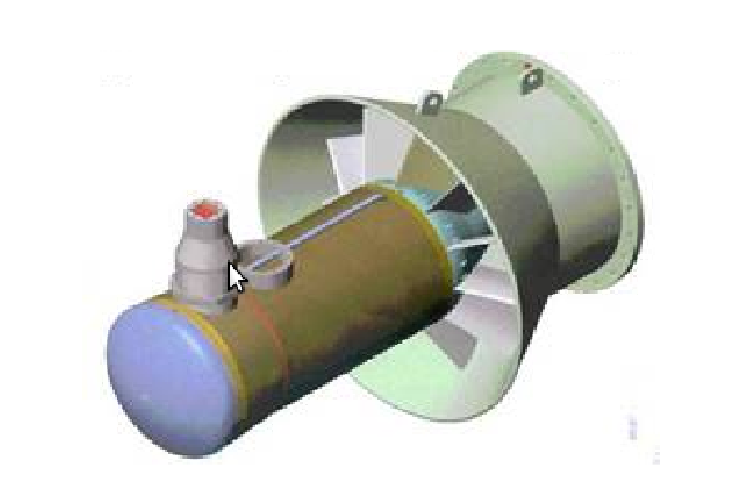
\includegraphics{Matrix2.eps}}
\end{minipage}
\caption{Matrix turbine and its main hydraulic parts. }
\label{Matrix_c}
\end{figure}

Hydromatrix$\circledR$ ability to use existing weir structures reduces additional civil works to minimum and enables power plant operators to install hydroelectric power plants at extremely competitive costs with minimal environmental im-pact. The number of matrix turbines and their arrangement in rows depends on the existing civil structure and its position relative to the head- and tail-water elevations. The use of a number of small turbine generator units (also known as “modules”) results in simple and robust turbine and generator design. The standardized modular factory assembled grid or “matrix” ( fig.~\ref{Matrix_a}) results in short project schedules and high availability. A Hydromatrix$\circledR$ turbine consists of three different parts (fig.\ref{Matrix_c}). The distributor cone containing the stay-wanes, the runner and the draft-tube.



\begin{figure}[h!]
\begin{minipage}[b]{0.5\linewidth}
 \centering
 \resizebox*{7.0cm}{!}{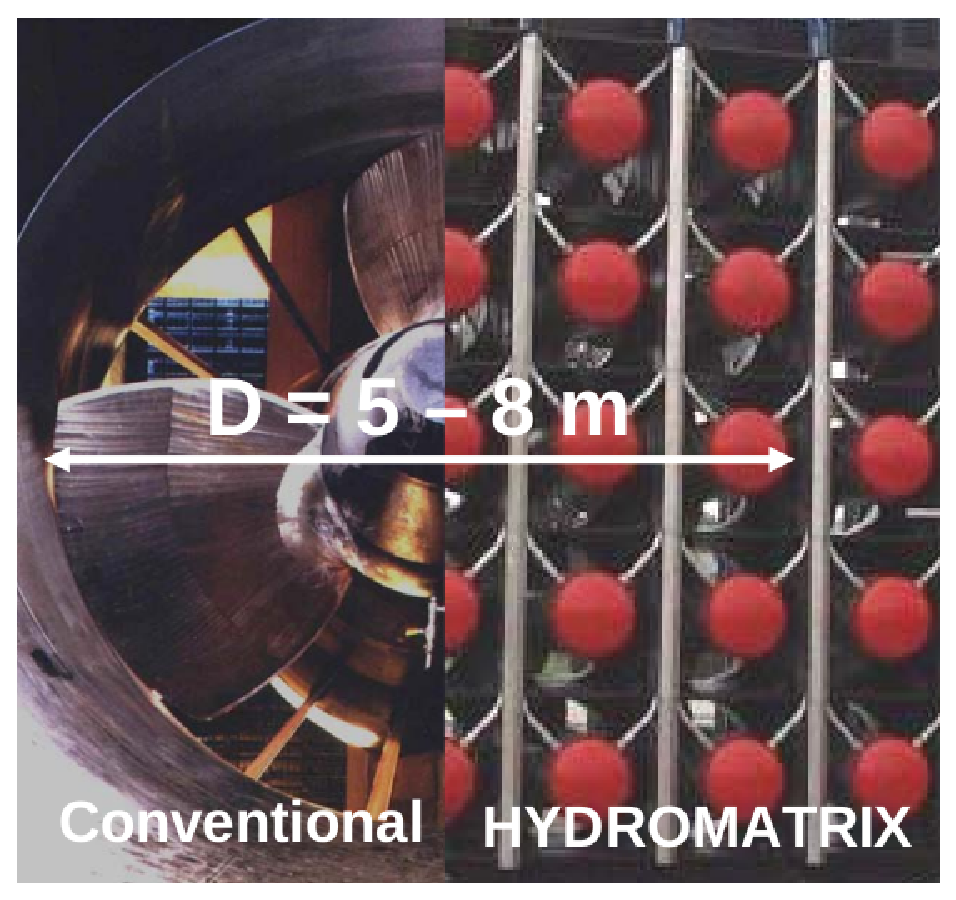
\includegraphics{Matrix3.eps}}
\end{minipage}
\begin{minipage}[b]{0.5\linewidth}
 \centering
 \resizebox*{7.0cm}{!}{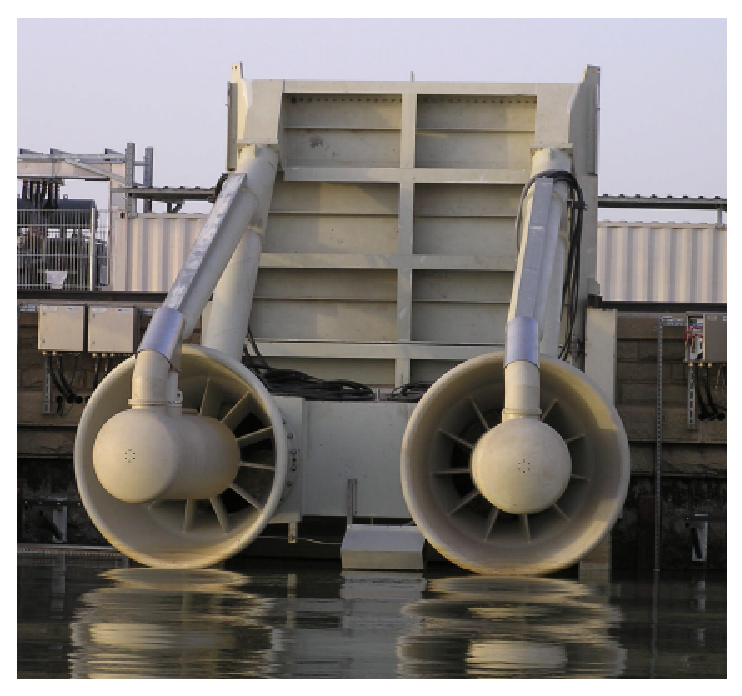
\includegraphics{Matrix4.eps}}
\end{minipage}
\caption{Left; replacement of a single large turbine by a matrix of smaller ones. Right; Matrix turbines in raised position (in case of flood conditions, inspection or maintenance).}
\label{Matrix_a}
\end{figure}

In order to achieve technical and economical feasible applications, the following main conditions have to be observed; 
\begin{itemize}
\item Available plant discharge from ~ $100 m^3/s$; 
\item Available head from 3 m up to 30 m; 
\item Minimum submergence 1.5 m below tailwater;
\item Unit output from 200 kW up to ~ 700 kW ;
\item Close grid connection ;
\item Structure available $\&$ suitable for HYDROMATRIX $\circledR$; 
\begin{itemize}
	\item Navigation dams; Large Lock $\&$ Dams navigational structures along a number of major rivers. 
	\item Irrigation dams; Many structures are existing for irrigation purposes worldwide, spilling water to agricultural areas on a regular basis.
	\item Sluice in shiplocks; Navigation river systems include dams and locks for ship transfer. Where an existing slot is available, a HYDROMATRIX $\circledR$ module can be installed for power generation. The turbine-generator units can be specifically designed to operate in both flow directions. Due to low operating heads feasibility has to be checked carefully. 
	\item Abandoned shiplocks; Due to increasing navigation and transport activities on major rivers the original shiplocks have become too small and new shiplocks were built.
\end{itemize}
\end{itemize}


\section{Case formulation}
The design problem in hand consists of the design of the rotor blades, rotor hub and stay-vanes end-tips. Distributor cone, runner shroud and draft tube are fixed due to the pre-constructed modular contraction and the generator size (fig.\ref{Matrix_b}).     


\begin{figure}[h!]
\centering
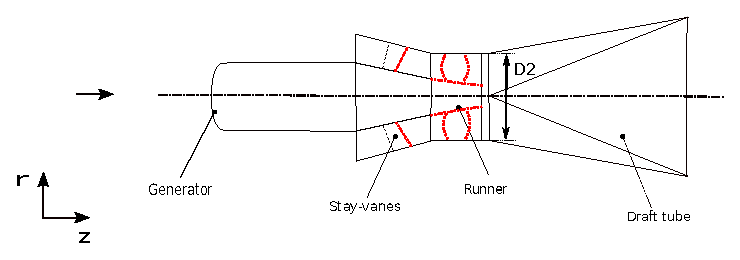
\includegraphics[width=120mm]{gen_turb.eps}    
\caption{Matrix turbine schematic representation, with red are the free to design parts and black are the fixed due to construction constraints parts.  }
\label{Matrix_b}
\end{figure}

\subsection{Design parameterization}
The design vector in this case is split into 2 parts, one responsible for runner blade and hub and one for the stay-vanes. The first part is based on the general parameterization and is uses $nvar$ design variables to describe the rotor blades mean surface, thickness distribution and hub generatrices (table. \ref{design_vars2}). Second part of the parameterization is the part responsible for the stay-vanes TE, stay-vanes thickness distributions are frozen due to structural reasons (stay-vanes have to hold both the generator and runner weight in place) and stay-vane LE is fixed since the flow meats the stay-vanes with an axial velocity.       

\begin{table}[h!]
\begin{center}
\begin{tabular}{ |c|l| }
\hline

Number of              & Design variables determining the:\\
design variables       & \\
\hline
n & spanwise distributions of $\theta_{LE}$\\
\hline
n & spanwise distributions of $\theta_{TE}$\\
\hline
n & spanwise distributions of $\beta_{LE}$\\
\hline
n & spanwise distributions of $\beta_{TE}$\\
\hline
n & spanwise distributions of $\zeta_{LE}$\\
\hline
n & spanwise distributions of $\zeta_{TE}$\\
\hline
n & spanwise thickness distributions for PS \\
\hline
n & spanwise thickness distributions for SS\\
\hline
n & LE meridional position\\
\hline
n & TE meridional position\\
\hline
n & Shroud meridional generatrices \\
\hline
n & Hub meridional generatrices\\
\hline
$n x 11$ & chordwise thikness destribution for PS (11 profiles)\\
\hline
$n x 11$ & chordwise thikness destribution for SS (11 profiles)\\
\hline
\hline
nvar & Design variables, in total \\
\hline   
\end{tabular}
\caption{
The $nvar$ design variables used to parameterize the Matrix runner.}
\label{design_vars2}
\end{center}
\end{table}

   


\subsection{Objectives $\&$ Constraints}

%\begin{figure}[h!]
%\centering
%\includegraphics[width=100mm]{matrix.eps}    
%\caption{Hydromatrix$circledR$: in case of flood conditions, inspection or maintenance, some or all of %the modules can easily be removed using a small crane.}. 
%}
%\label{Matrix2}
%\end{figure}

\section{Parametric study}
\subsection{Initial design}
\subsubsection{EA}
\subsubsection{EA(KBS)}
\subsubsection{Discussion}
\subsection{Refinement}
\subsubsection{EA (SBX)}
\subsubsection{MAEA (SBX)}
\subsubsection{MAEA (PCA)}
\subsubsection{MAEA (SOM)}
\subsubsection{Discussion}
\section{Final methodology}
% ---------------------------------------------------------------------------
% ----------------------- end of thesis sub-document ------------------------
% ---------------------------------------------------------------------------